\documentclass{article}
\usepackage[legalpaper, portrait, margin=1.25in]{geometry}
\usepackage{amsthm}
\usepackage{amsmath}
\usepackage{amsfonts}
\usepackage{amssymb}
\usepackage{amsrefs}
\usepackage[utf8]{inputenc}
\usepackage{titling}
\usepackage{scrextend}
\usepackage{url}
\usepackage{microtype}
\usepackage{svg}
\usepackage{shellesc}
\usepackage{setspace}

\newenvironment{Figure}
  {\par\medskip\noindent\minipage{\linewidth}}
  {\endminipage\par\medskip}

\usepackage{multicol, caption}

\title{Piecewise Polynomials \\
    {\large Real Analysis II Investigation Assignment}}
\author{Lucas LaValva}
\date{\today}


\usepackage{fancyhdr}
\pagestyle{fancy}
\lhead{\theauthor}
\rhead{Investigation Assignment}

\begin{document}
\maketitle

\doublespacing

\begin{abstract}
    This paper is a discussion of the various methods that can be used to interpolate through a set of points to approximate a function. Three functions are observed; Polynomial Inpterpolation, Linear Interpolation, and Cubic Spline Interpolation. In analysis of these functions, we will find reasonable error bounds and discuss the benefits and drawbacks of each.
\end{abstract}

\section{Introduction}

The rapid improvements in computation throughout the past fifty years have opened many doors for mathematicians, and given them the opportunity to approach problems from a radically different angle. In addition, this new perspective has enflamed many classes of problems that had not previously been explored heavily. Two topics that frequently pertain to computational mathematics are compression of data and, more obviously, efficiency of computation. The compression of complicated mathematical constructs into smaller amounts of information is more often than not an exploration of the tradeoff between ``amount of information'' and the accuracy of what that information represents.

With current algorithms and technology, triginometric functions are computationally expensive to calculate. As such, many programs that require large volumes of triginometry keep a table of approximate values and refer to it instead of doing computations on the fly. As demand for precision increases, the size of this table must also increase rapidly. Therefore, other options have been considered for fast calculation of sine. One such method is polynomial interpolation.

\section{Polynomial Interpolation}
\label{section:polynomial_interpolation}

Polynomial interpolation \cite{enwiki:polynomial_interpolation} is a method for generating an infinitely differentiable function that passes through a one-to-one set of points in $\mathbb{R}_2$. In the examples below, evenly spaced points are placed on a sine curve and polynomials are constructed to pass through each of those points (depicted in black).

\medbreak
\centerline{
    \begin{minipage}{0.3\textwidth}
        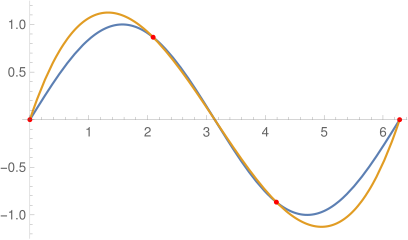
\includegraphics[width=\linewidth]{Images/SineInterpolation_EvenlySpaced/sin_interpolation_4.png}
        \captionsetup{justification=centering}
        \captionof{figure}{\\ 4 evenly spaced points}
    \end{minipage}
    \begin{minipage}{0.3\textwidth}
        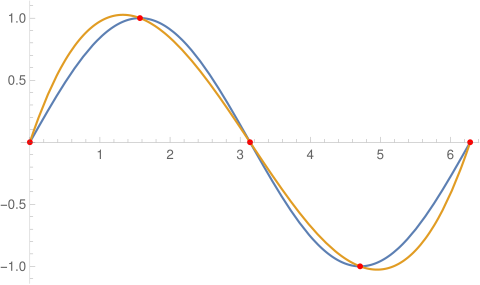
\includegraphics[width=\linewidth]{Images/SineInterpolation_EvenlySpaced/sin_interpolation_5.png}
        \captionsetup{justification=centering}
        \captionof{figure}{\\ 5 evenly spaced points}
    \end{minipage}
    \begin{minipage}{0.3\textwidth}
        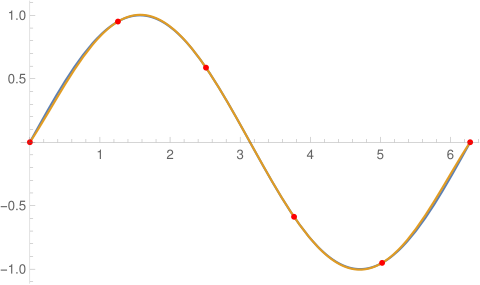
\includegraphics[width=\linewidth]{Images/SineInterpolation_EvenlySpaced/sin_interpolation_6.png}
        \captionsetup{justification=centering}
        \captionof{figure}{\\ 6 evenly spaced points}
    \end{minipage}
}
\medbreak
\subsection{Lagrange Interpolation}

These polynomials are calculated using a method called \textbf{Lagrange Interpolation} \cite{enwiki:lagrange_polynomial}\cite{mathworld:lagrange_polynomial}. To preform this method, we begin with $n$ data points that will be referred to as $(x_1, y_1), (x_2, y_2), \ldots, (x_n, y_n)$. In order to find a polynomial that passes through all of these points, we use
\begin{equation}
    P(x) = \sum_{j=1}^n\left(y_j\prod_{\substack{k=1 \\ k\neq j}}^n \frac{x-x_k}{x_j-x_k} \right)
\end{equation}
or, written more explicitly,
\begin{align*}
      & y_1\frac{(x-x_2)(x-x_3)\ldots(x-x_n)}{(x_1-x_2)(x_1-x_3)\ldots(x_1-x_n)}          \\
    + & y_2\frac{(x-x_1)(x-x_3)\ldots(x-x_n)}{(x_2-x_1)(x_2-x_3)\ldots(x_2-x_n)}          \\
      & \vdots                                                                            \\
    + & y_n\frac{(x-x_1)(x-x_2)\ldots(x-x_{n-1})}{(x_n-x_1)(x_n-x_2)\ldots(x_n-x_{n-1})}.
\end{align*}
In most cases, this formula works very well. In fact, at each interpolation point the accuracy is perfect, so as the number of points tends towards infinity the error must approach 0. In practice, however, it is not possible to apply this formula to an infinite number of points so it is important to ensure that the error with a finite number of points is reasonable. This is why it is worth discussing certain circumstances where significant error occurs.

\subsection{Runge's Phenomenon}

In the generation of Fourier series, it is commonly known that if the function is discontinuous then it is not unlikely to find fluctuations of increasing magnitude on the Fourier approximation around the point at which discontinuity occurs. This is known as \textbf{Gibbs Phenomenon}, and it is apparent in situations such as an approximation of the sawtooth wave, or the periodic projection of $f(x)=x$. The Fourier series of a sawtooth wave can be represented as
\[
    S_n = \sum_{m=1}^{n}\frac{-2(-1)^{m}}{m}\sin(mx).
\]
Figure \ref{fig:sawtooth_gibbs} shows the sawtooth wave (represented in black) as well as its Fourier series when $n=1, 3, 9, 27$ and $81$ (orange, green, purple, blue, and red, respectively)

\medbreak
\centerline{
    \begin{minipage}{0.4\textwidth}
        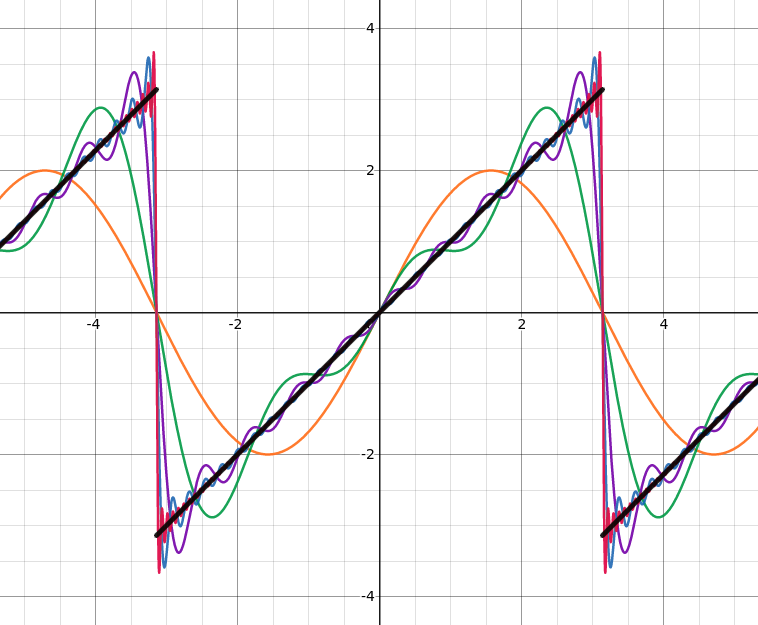
\includegraphics[width=\linewidth]{Images/gibbs.png}
        \captionsetup{justification=centering}
        \captionof{figure}{\\ Fourier Series of Sawtooth Wave}
        \label{fig:sawtooth_gibbs}
    \end{minipage}
}
\medbreak

As can be seen in Figure \ref{fig:sawtooth_gibbs}, $S_{81}$ is very close to the goal function everywhere except around the point of discontinuity.

A similar phenomenon exists for Lagrange interpolation, but because a set of points is inherently discontinuous it does not make sense to describe ``points of discontinuity.'' Instead, the equivalent of the Gibbs phenomenon for Lagrange interpolation occurs for functions that have a unique shape. In 1901, Carl David Runge discovered that for the function (known as the \textbf{Runge Function}) % TODO: `\cite{enwiki:runge_phenomenon}` breaks the ENTIRE bib for some reason
\begin{equation}
    f(x)=\frac{1}{1+25x^2},
    \label{eq:runge_function}
\end{equation}
Lagrangian interpolation creates some interesting results (shown below).

\medbreak
\centerline{
    \begin{minipage}{0.3\textwidth}
        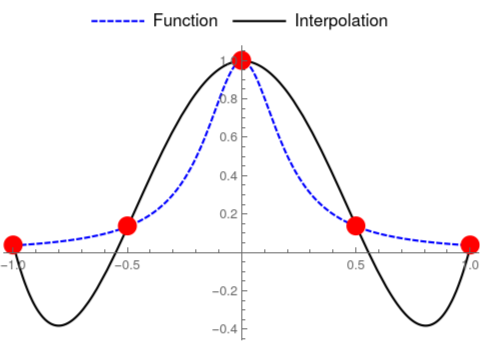
\includegraphics[width=\linewidth]{Images/RungeInterpolation_EvenlySpaced/runge_interpolation_5.png}
        \captionsetup{justification=centering}
        \captionof{figure}{\\ 5 evenly spaced points}
        \label{fig:runge_evenlyspaced_5}
    \end{minipage}
    \begin{minipage}{0.3\textwidth}
        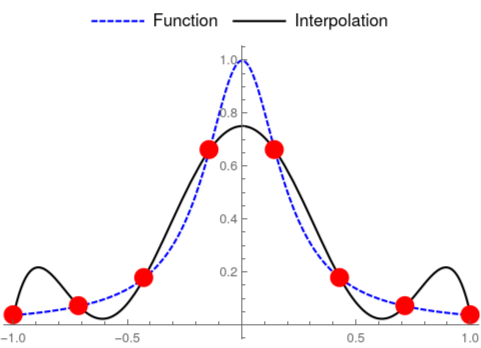
\includegraphics[width=\linewidth]{Images/RungeInterpolation_EvenlySpaced/runge_interpolation_8.png}
        \captionsetup{justification=centering}
        \captionof{figure}{\\ 8 evenly spaced points}
    \end{minipage}
    \begin{minipage}{0.3\textwidth}
        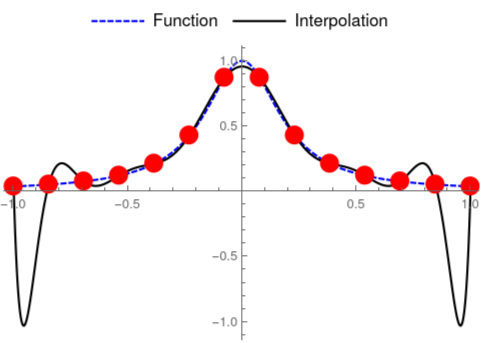
\includegraphics[width=\linewidth]{Images/RungeInterpolation_EvenlySpaced/runge_interpolation_14.png}
        \captionsetup{justification=centering}
        \captionof{figure}{\\ 14 evenly spaced points}
        \label{fig:runge_evenlyspaced_14}
    \end{minipage}
}
\medbreak

The heavy oscillation around the edges of this function is commonly known as \textbf{Runge's Phenomenon}. With the identification of this problem, it is worth exploring the possibility of measuring the magnitude at which the error occurs.

\subsection{Interpolation Error}


One way to record the amount of error that is generated by this function is by finding the largest amount of distance between the actual function $f$ and its interpolating polynomial $P_n$ using
\begin{equation}
    E_{\max}=\lVert f(x)-P_n(x)\rVert_\infty
\end{equation}

To find a method for generating $f(x)-P_n(x)$, we can consider a function
\begin{equation}
    \phi(t) = f(t) - P_n(t) - \left(\frac{f(x)-P_n(x)}{\prod_{k=1}^n(x-x_k)}\right)\prod_{k=1}^n(t-x_k)
\end{equation}
Let us consider the case of $\phi(x_i)$, where $1\leq i\leq n$ and $i\in\mathbb{Z}$.\cite{youtube:interpolation_error} Because of the properties of interpolating polynomials, we know that $f(x_i)-P_n(x_i)$ must be 0. On top of this, we can be certain that within the product $\prod_{k=1}^n(x_i-x_k)$ there must be some point at which $i=k$, and thus the product is 0. Therefore, we know that for all $i$, $\phi(x_i)=0$. Thus, there are at least $n$ points at which $\phi(t)$ vanishes.

In addition, we can consider the case of $\phi(x)$. Because both products are the same, this simplifies to
\begin{align*}
    \phi(x) & = (f(x)-P_n(x)) - (f(x)-P_n(x)) \\
            & = 0
\end{align*}
This tells us that there are at least $n+1$ points at which $\phi(t)$ vanishes.

Rolle's theorem states that if a function has $N$ zeroes in a given domain, then the derivative of that function has $N-1$ zeroes. Thus, there are $n$ points at which $\phi'(t)$ vanishes. We can apply this theorem in succession $n$ times to see that $\phi^{(n)}(t)$ vanishes at some point
$\xi$ in the function's domain. We compute
\begin{equation*}
    \phi^{(n)}(x) = f^{(n)}(t) - P_n^{(n)}(t) - \left(\frac{f(x)-P_n(x)}{\prod_{k=1}^n(x-x_k)}\right)\frac{d^n}{dt^n}\prod_{k=1}^n(t-x_k).
\end{equation*}
Because $P_n$ is a polynomial of \textit{at most} $n-1$, we know that $P_n^{(n)}(t)=0$. We also know that $\prod_{k=1}^n(t-x_k)$ consists of a polynomial in which the highest power is $t^n$, so
\[
    \frac{d^n}{dt^n}\prod_{k=1}^n(t-x_k)=n!.
\]
Therefore, we can use the fact that $\phi^{(n)}(\xi)=0$ and rearrange the equation to show that
\[
    0 = f^{(n)}(\xi) - (0) - \left(\frac{f(x)-P_n(x)}{\prod_{k=1}^n(x-x_k)}\right)n!
\]
and thus
\[
    f(x)-P_n(x) = \frac{f^{(n)}(\xi)}{n!}\prod_{k=1}^n(x-x_k).
\]
Therefore, the maximum error can be calculated using
\[
    E_{\max} = \left\lVert\frac{f^{(n)}(\xi)}{n!}\prod_{k=1}^n(x-x_k)\right\rVert_\infty
\]
where $\xi$ is in the domain of the function. (Note: Most resources online start indexing points at $x_0$ instead of $x_1$, so an additional differentiation is required. I have chosen to keep it this way against convention because I think it makes the equations cleaner and easier to understand.)

When points are equally spaced, as they have been thus far in this analysis, we can simplify the error equation using the fact that in a domain $[a, b]$, $x_k=a+kh$ where $h=\frac{b-a}{n-1}$. Then the product in the interpolation can be bounded to
\begin{align*}
    \left|\prod_{k=1}^n(x-x_k)\right| & = \prod_{k=1}^n|x-x_k|              \\
                                      & \leq \frac{(n-1)!(b-a)^n}{4(n-1)^n} \\ % TODO: Understand and explain this step
                                      & \leq \frac{(n-1)!}{4}h^n.
\end{align*}
Therefore, the error can be bounded by
\begin{align*}
    E_{\max} & = \left\lVert\frac{f^{(n)}(\xi)}{n!}\prod_{k=1}^n(x-x_k)\right\rVert_\infty                                       \\
             & \leq \frac{\left\lVert f^{(n)}(\xi)\right\rVert_{\infty}}{n!}\left\lVert\prod_{k=1}^n(x-x_k)\right\rVert_{\infty} \\
             & \leq \frac{\left\lVert f^{(n)}(\xi)\right\rVert_{\infty}}{n!}\left\lVert\frac{(n-1)!}{4}h^n\right\rVert_{\infty}  \\
             & = \frac{\left\lVert f^{(n)}(\xi)\right\rVert_{\infty}h^n}{4n}
\end{align*}
for evenly spaced points.

For many commonly used functions, such as $\sin(x)$ and $\cos(x)$, $E_{\max}$ quickly approaches 0 as $n\to\infty$. However, equation \eqref{eq:runge_function} does not behave in this way. As $n$ grows larger,
\[
    \left\lVert\frac{d^n}{dx^n}\frac{1}{1+25x^2}\right\rVert_\infty > \frac{h^n}{4n}
\]
and
\[
    \frac{h^n}{4n}\left\lVert\frac{d^n}{dx^n}\frac{1}{1+25x^2}\right\rVert_\infty\to\infty.
\]
As a result, the error continues to worsen as the number of points increases.

This finding tells us that the most likely place to find error in polynomial interpolation is for functions with which each derivative is much larger than the one before it. As a simple example, let us view the linear polynomial interpolation for $f(x)=e^{x^2}$ (Rightmost point excluded, because it is out of range):

\medbreak
\centerline{
    \begin{minipage}{0.4\textwidth}
        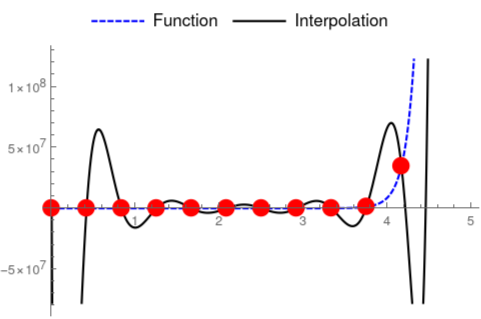
\includegraphics[width=\linewidth]{Images/EXSquaredInterpolation_EvenlySpaced/exsquared_interpolation_13.png}
        \captionsetup{justification=centering}
        \captionof{figure}{\\ 13 evenly spaced points $\left(e^{x^2}\right)$}
    \end{minipage}
}
\medbreak

There are various appraches that can be taken in order to remedy this problem. Since the error tends to occur around the edges of the domain, one such approach could be to consider spacing points so that there are more around the edges, instead of evenly distributing them throughout the domain.

\subsection{Chebyshev Nodes}

To decide where exactly to place the points, recall that the error is bound in part by
\[
    \left\lVert\prod_{k=1}^n(x-x_k)\right\rVert_{\infty}.
\]
Thus, one way to minimize error is to find a way to shrink this product.

To begin, let us consider a monic polynomial $T_n(x)$ whose zeroes are $x_1, x_2, \ldots, x_n$. This polynomial can be written as
\begin{equation}
    T_n(x) = (x-x_1)(x-x_2)\ldots(x-x_n)
\end{equation}
It can be shown that
\[
    \min_{x\in[-1, 1]}\lVert T_n(x)\rVert_\infty = \frac{1}{2^n},
\]
and that this is acheived when the $x$ values of the interpolation points are spaced so that a circle of radius 1 would have them evenly spaced. This is demonstrated in Figure \ref{fig:chebyshev_semicircle}. \cite{enwiki:chebyshev_nodes}

\medbreak
\centerline{
    \begin{minipage}{0.4\textwidth}
        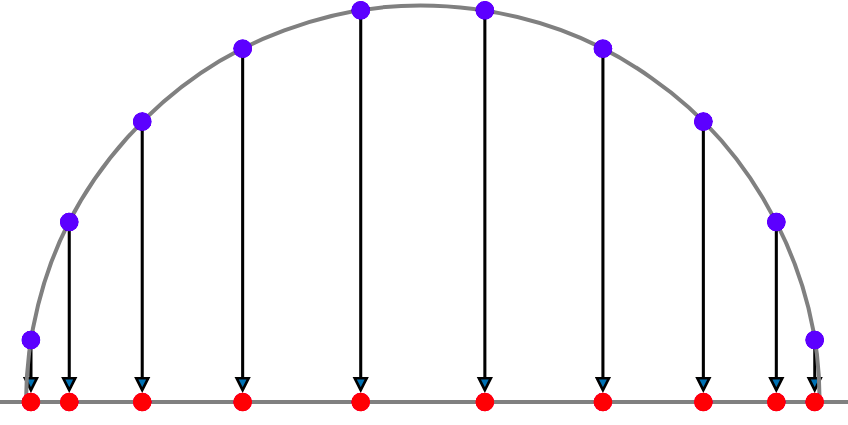
\includegraphics[width=\linewidth]{Images/chebyshev_semicircle.png}
        \captionsetup{justification=centering}
        \captionof{figure}{\\ Spacing of $x$ values}
        \label{fig:chebyshev_semicircle}
    \end{minipage}
}
\medbreak

In algebraic terms, for any domain $[a, b]$
\begin{equation}
    x_k = \cos\left(\frac{2\pi(n-k)}{2n+1}\right)
\end{equation}
These sets of points are known as \textbf{Chebyshev nodes}.

The benefit of using Chebyshev nodes to select interpolation points is very visibly evident for functions that are generally victims of  Runge's phenomenon. For example, here are the Chebyshev nodes for Figure \ref{fig:runge_evenlyspaced_5}-\ref{fig:runge_evenlyspaced_14}:

\medbreak
\centerline{
    \begin{minipage}{0.3\textwidth}
        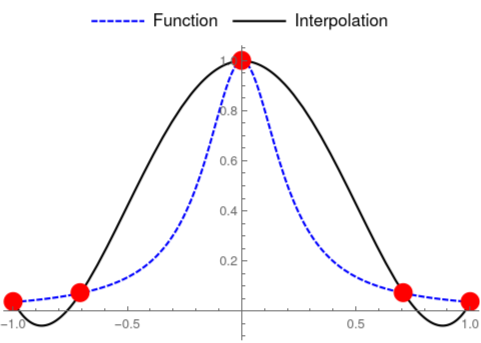
\includegraphics[width=\linewidth]{Images/RungeInterpolation_Chebyshev/runge_interpolation_5.png}
        \captionsetup{justification=centering}
        \captionof{figure}{\\ 5 Chebyshev points}
    \end{minipage}
    \begin{minipage}{0.3\textwidth}
        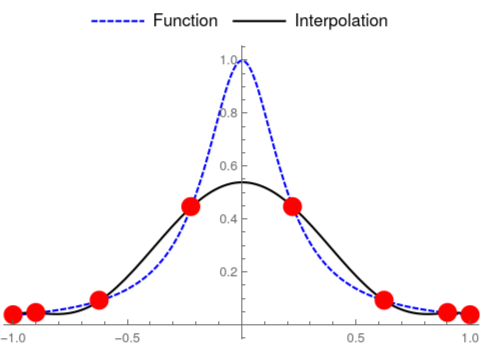
\includegraphics[width=\linewidth]{Images/RungeInterpolation_Chebyshev/runge_interpolation_8.png}
        \captionsetup{justification=centering}
        \captionof{figure}{\\ 8 Chebyshev points}
    \end{minipage}
    \begin{minipage}{0.3\textwidth}
        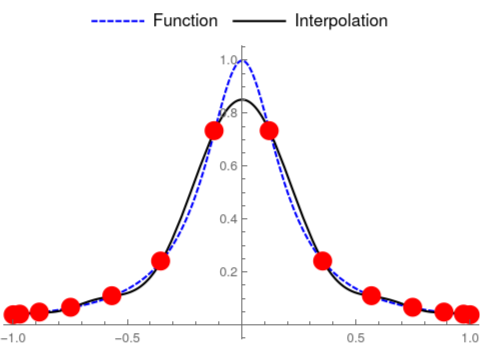
\includegraphics[width=\linewidth]{Images/RungeInterpolation_Chebyshev/runge_interpolation_14.png}
        \captionsetup{justification=centering}
        \captionof{figure}{\\ 14 Chebyshev point)}
    \end{minipage}
}
\medbreak

While Chebyshev nodes are the most effective approach for minimizing error between a single polynomial that passes through points on a function, it is not necessarily the most effective method for approximating a function based only on a set of points.

\section{Piecewise Interpolation}

\subsection{Linear Interpolation}

In cases like Figure \ref{fig:runge_evenlyspaced_5} and Figure \ref{fig:runge_evenlyspaced_14}, where the Runge phenomenon has a large effect or where the polynomial drifts far away from the function between points, one might imagine that the function could be approximated more reasonably by simply drawing lines between each of the points. This is known as \textbf{Linear Interpolation}, and for a set of $n$ locations $x_k$ and it can be written as
\[
    P(t) = \begin{cases}
        y_1 + (y_2-y_1)\frac{t-x_1}{x_2-x_1}                 & x_1 < t < x_2     \\
        y_2 + (y_3-y_2)\frac{t-x_2}{x_3-x_2}                 & x_2 < t < x_3     \\
        \vdots                                                                   \\
        y_{n-1} + (y_n-y_{n-1})\frac{t-x_{n-1}}{x_n-x_{n-1}} & x_{n-1} < t < x_n \\
    \end{cases}
\]
where $y_k=f(x_k)$.

While linear interpolation is fast to compute and easy to understand, there are a myriad of disatvantages. The result is a continuous function, but it is not differentiable except in the linear case and it allows a large amount of error in between each set of points.

To calculate error in linear interpolation, we begin with a twice continuously differentiable function $f$ and its linear interpolation $P$, and select some $x$ between $x_a$ and $x_b$. Then
\[
    f(x)-P(x) = \frac{(x-x_a)(x-x_b)}{2}f''(c_x)
\]
for some $c_x\in[x_a, x_b]$. Therefore, we can define an error bound
\begin{align*}
    E_{\max} & = |f(x)-P(x)|                                             \\
             & \leq \frac{(x-x_a)(x-x_b)}{2}\lVert f''(x)\rVert_{\infty} \\
             & \leq \frac{(x_b-x_a)^2}{8}\lVert f''(x)\rVert_{\infty}.
\end{align*}
This tells us that the error is proportional to the square of the distance between data points, and that a function whose second derivative has a high sup norm is more likely to have a large interpolation error. \cite{enwiki:interpolation}\cite{enwiki:linear_interpolation} This is wonderfully apparent in visualizations of the sine curve, which has a second derivative equal to itself. As is shown in Figure \ref{fig:linear_sine_6} and Figure \ref{fig:linear_sine_9}, error between the sine curve and its linear interpolation tends to be larger when $|\sin(x)|$ is larger.

\medbreak
\centerline{
    \begin{minipage}{0.4\textwidth}
        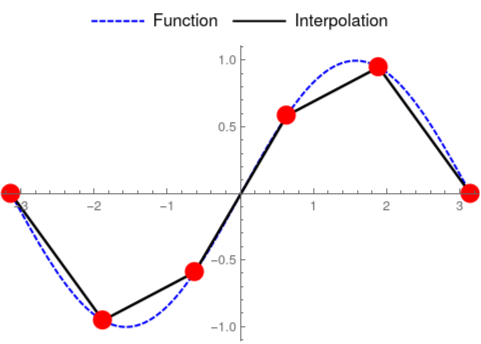
\includegraphics[width=\linewidth]{Images/LinearInterpolation/sine_6.png}
        \captionsetup{justification=centering}
        \captionof{figure}{\\ 6 evenly spaced points}
        \label{fig:linear_sine_6}
    \end{minipage}
    \begin{minipage}{0.4\textwidth}
        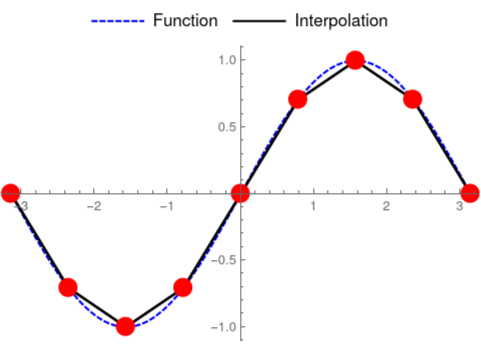
\includegraphics[width=\linewidth]{Images/LinearInterpolation/sine_9.png}
        \captionsetup{justification=centering}
        \captionof{figure}{\\ 9 evenly spaced points}
        \label{fig:linear_sine_9}
    \end{minipage}
}
\medbreak

Of course, the drawbacks of linear interpolation have inspired generalizations which have a lower margin of error, and potentially those which are continuously differentiable. One such method of generalization is to design an single function interpolation which is guaranteed to make contact with each point. This was explored in Section \ref{section:polynomial_interpolation}, with the use of polynomial interpolation. In light of Runge's phenomenon and similar errors in this method, one might consider some of the benefits that the piecewise nature of linear interpolation has to offer. If each segment was still assigned its own function, but this function took more than just its adjacent points into consideration, then polynomials could stay in lower order while still approximating the curves of the approximation function. This structure is known as a \textbf{Polynomial Spline}.

\subsection{Polynomial Splines}

In order to acheive the desired effect, any generated interpolation for the function $f(x)$ and set of $n$ values $x_k$ should
\begin{enumerate}
    \item make contact with each point $(x_k, f(x_k))$,
    \item have a lower margin of error than linear interpolation, and
    \item allow for continuous differentiability.
\end{enumerate}

Most graphics programs and numerical analysts have settled on polynomials of order 3. This is because they allow for the function to be twice continuously differentiable, provide a fairly small margin of error, and are straightforward to calculate.

\subsection{Cubic Splines}

A cubic spline $S_n(x)$ satisfies the following properties:
\begin{align}
    S_n(x_k)                    & = f(x_k)                      \\
    \lim_{x\to x_i^-}S_n'(x_k)  & = \lim_{x\to x_i^+}S_n'(x_k)  \\
    \lim_{x\to x_i^-}S_n''(x_k) & = \lim_{x\to x_i^+}S_n''(x_k) \\
    S_n''(x_0) z = S_n''        & (x_n) = 0
    \label{eq:zero_at_endpoints}
\end{align}

To begin with the construction of a cubic spline, let us introduce variables $M_0, \ldots, M_n$ such that
\[
    M_k\equiv S_n''(x_k), k\in \mathbb{Z}_n
\]
Because $S_n(x)$ is a cubic spline on $[x_{k-1}, x_k]$, we know that its second derivative is linear. Thus, $S_n''(x)$ can be calculated based on its values at each endpoint via \textit{linear interpolation}! Then for $x\in[x_{k-1}, x_k]$,
\begin{equation}
    S_n''(x) = M_{k-1}\frac{x_k-x}{x_k-x_{k-1}}+M_k\frac{x-x_{k-1}}{x_k-x_{k-1}}.
\end{equation}
Therefore, we can find that
\begin{align*}
    S_n'(x) & = \int S_n''(x)dx                                                                            \\
            & = -M_{k-1}\frac{(x_k-x)^2}{2(x_k-x_{k-1})} + M_k\frac{(x-x_{k-1})^2}{2(x_k-x_{k-1})} + A     \\
    S_n(x)  & = \int S_n'(x)dx                                                                             \\
            & = M_{k-1}\frac{(x_k-x)^3}{6(x_k-x_{k-1})} + M_k\frac{(x-x_{k-1})^3}{6(x_k-x_{k-1})} + Ax + B
\end{align*}
Denote $y_k=f(x_k)$. Then we can assert that
\[
    S_n(x_{k-1})=y_{k-1}, S_n(x_k)=y_k.
\]
For simplicity, let $h_k=x_k-x_{k-1}$. After substituting values for $A$ and $B$ \cite{Jameson}, we find that
\begin{align}
    S_n(x)  & = M_{k-1}\frac{(x_k-x)^3}{6h_k} + M_k\frac{(x-x_{k-1})^3}{6h_k} \nonumber                                                         \\
            & \phantom{=} + \left(y_{k-1}-M_{k-1}\frac{h_k^2}{6}\right)\frac{x_k-x}{h_k} + \left(y_k+M_k\frac{h_k^2}{6}\right)\frac{x-x_k}{h_k} \\
    S_n'(x) & = -M_{k-1}\frac{(x_k-x)^2}{2h_k} + M_k\frac{(x-x_{k-1})^2}{2h_k} + \frac{y_k-y_{k-1}}{h_k} - \frac{h_k(M_k-M_{k-1})}{6}
    \label{eq:first_derivative_cubic}
\end{align}
As a result of these calculations, we can be certain that both $S_n(x)$ and $S_n''(x)$ are continuous even across points. In order to acquire continuity for $S_n'(x)$, we can consider that
\begin{align*}
    S_n'(x_k^-) & = M_{k-1}\frac{h_k}{6}+M_k\frac{h_k}{3}+\frac{y_k-y_{k-1}}{h_k}             \\
    S_n'(x_k^+) & = M_k\frac{h_{k+1}}{3}+M_{k+1}\frac{h_{k+1}}{6}+\frac{y_{k+1}-y_k}{h_{k+1}}
\end{align*}
After setting these two equal and rearranging the equation, we are left with what seems to be a way to calculate each $M_k$ based on its neighbors.
\begin{equation}
    M_{k-1}\frac{h_k}{6} + M_k\frac{h_k+h_{k+1}}{3} + M_{k+1}\frac{h_{k+1}}{6} = \frac{y_{k+1}-y_k}{h_{k+1}} - \frac{y_k-y_{k-1}}{h_k}
    \label{eq:cubic_implosion}
\end{equation}
Recall from \eqref{eq:zero_at_endpoints} that $S_n''(x_k)=M_k=0$ at both endpoints of the domain $(k=0, n)$. Then we can use equation \eqref{eq:first_derivative_cubic} to find that
\begin{align*}
    M_1     & = \frac{6(y_1-y_0)}{h_1^2}     \\
    M_{n-1} & = \frac{6(y_n-y_{n-1})}{h_n^2}
\end{align*}
After calculating $M_{\{0,1, n-1, n\}}$, we can use the equality in equation \eqref{eq:cubic_implosion} to learn what the rest are from either end.

The result of this enormous calculation is a twice differentiable piecewise function which passes through a set of points without susceptibility to Runge's phenomenon. Approximations are displayed below.
\begin{align*}
    f(x)=\frac{1}{1+25x^2} &  & x\in[-1, 1]
\end{align*}
\centerline{
    \begin{minipage}{0.3\textwidth}
        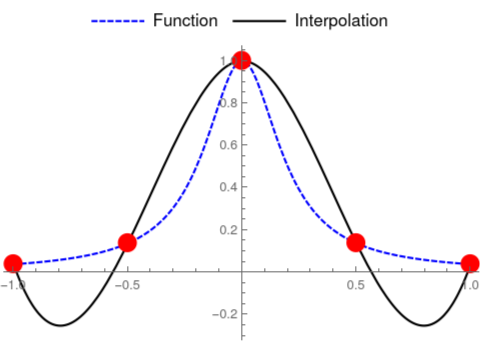
\includegraphics[width=\linewidth]{Images/RungeInterpolation_Cubic/runge_interpolation_5.png}
        \captionsetup{justification=centering}
        \captionof{figure}{\\ 5 evenly spaced points}
    \end{minipage}
    \begin{minipage}{0.3\textwidth}
        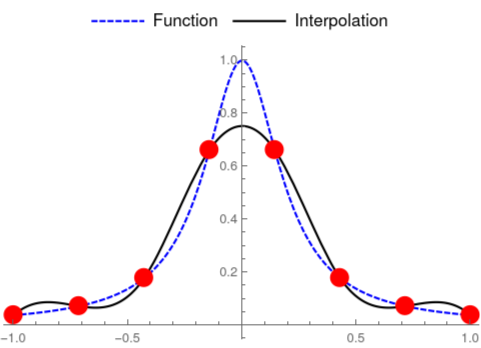
\includegraphics[width=\linewidth]{Images/RungeInterpolation_Cubic/runge_interpolation_8.png}
        \captionsetup{justification=centering}
        \captionof{figure}{\\ 8 evenly spaced points}
    \end{minipage}
    \begin{minipage}{0.3\textwidth}
        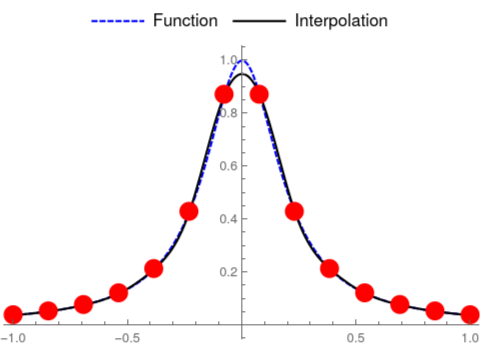
\includegraphics[width=\linewidth]{Images/RungeInterpolation_Cubic/runge_interpolation_14.png}
        \captionsetup{justification=centering}
        \captionof{figure}{\\ 14 evenly spaced points}
    \end{minipage}
}
\medbreak
\begin{align*}
    f(x) = \sin(x) &  & x\in[0, 2\pi]
\end{align*}
\centerline{
    \begin{minipage}{0.3\textwidth}
        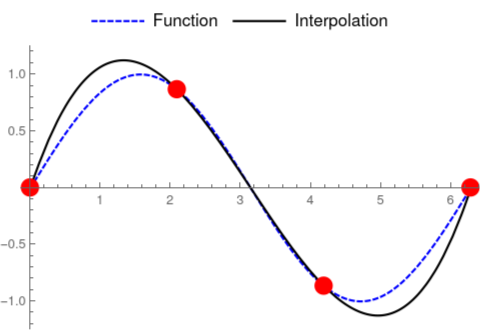
\includegraphics[width=\linewidth]{Images/SineInterpolation_Cubic/sin_interpolation_4.png}
        \captionsetup{justification=centering}
        \captionof{figure}{\\ 4 evenly spaced points}
    \end{minipage}
    \begin{minipage}{0.3\textwidth}
        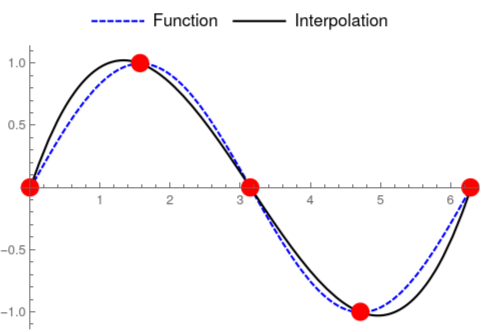
\includegraphics[width=\linewidth]{Images/SineInterpolation_Cubic/sin_interpolation_5.png}
        \captionsetup{justification=centering}
        \captionof{figure}{\\ 5 evenly spaced points}
    \end{minipage}
    \begin{minipage}{0.3\textwidth}
        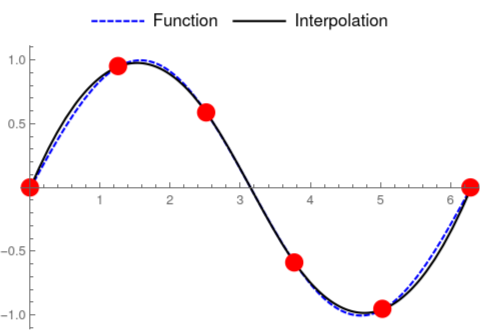
\includegraphics[width=\linewidth]{Images/SineInterpolation_Cubic/sin_interpolation_6.png}
        \captionsetup{justification=centering}
        \captionof{figure}{\\ 6 evenly spaced points}
    \end{minipage}
}
\medbreak

\section{Conclusion}

The material covered in this paper contains only a small slice of the research that has been done on the generation and optimization of interpolating functions. As has been shown, each method has its own benefits and drawbacks.

For a fast and easy to calculate approximation of a function, linear interpolation is ideal. However, this method is not differentiable and it does not handle functions with lots of curving very well. This interpolation is also not visibly appealing in many cases, because its lack of differentiability results in sharp changes in slope at each interpolation point.

One way to combat the drawbacks of linear interpolation is by interpolating a single polynomial over every interpolation point. This method has a straightforward equation and it usually approximates a function with a low error, but it is subject to Runge's phenomenon. However, this can be prevented by placing interpolation points on Chebyshev nodes instead of spacing them evenly throughout the function. One drawback of polynomial interpolation is that as the number of interpolation points increases, the degree of the polynomial increases as well. This results in some \textit{very} large polynomials that may take a long time for a computer to calculate.

Cubic spline interpolation, in many cases, seems to take the best elements from polynomial and linear inteprolation. A cubic spline is twice continuously differentiable, and for any given $x$ value only a single cubic function must be calculated. Because of these benefits, most computer programs that visualize interpolations use cubic splines in their calculations.


\bibliographystyle{acm}
\bibliography{investigationAssignment}

\end{document}